\section{Flood Fill}
\index{flood fill}

This is an algorithm that will, given some starting node(s), proceed to explore an entire graph by 'spreading' in all directions, hence, its name.
A sort of boundary can also be applied to limit the extent of 'flooding' the algorithm does.
More specifically, it can be used to 'color' or mark nodes in a certain manner.
It can be seen as a more specific example of breadth- or depth-first search.
A flood fill can be implemented with either a queue or a stack and runs in $O(n)$ time.

\begin{figure}[h]
    \centering
    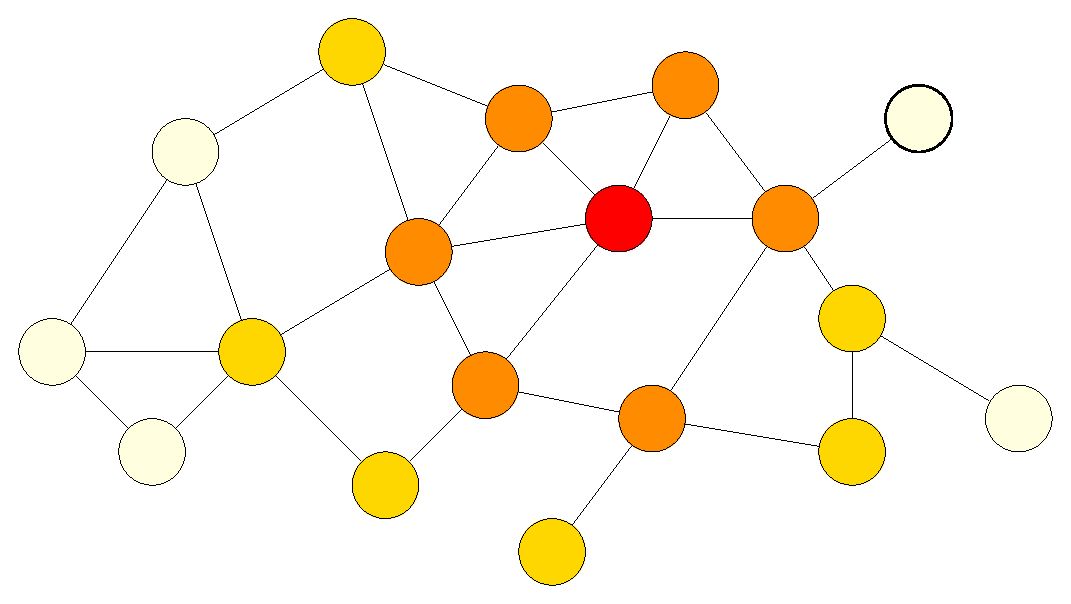
\includegraphics[width=0.6\textwidth]{./algorithms/flood-fill/partial-ff}
    \caption{\small A complete flood fill on a graph.
      The red node is where the algorithm started.
      Nodes visited later in the algorithm are progressively more yellow.}
\end{figure}
